\documentclass[12pt,a4paper]{article}
\usepackage[utf8]{inputenc}
\usepackage[T2A]{fontenc}
\usepackage[english,russian]{babel}
\usepackage[a4paper, mag=1000, left=1.5cm, right=2cm, top=2cm, bottom=2cm, headsep=0.7cm, footskip=1cm]{geometry}
\usepackage{amsmath}
\usepackage{pgfplots, colortbl}
\usepackage{makecell}
\usepackage{multicol}
\usepackage{pgfplotstable}
\pgfplotsset{compat=1.16}
\usepackage{minted}
\usepackage{listings}
\usepackage{lstfiracode}
\usepackage{caption}
\usepackage{mathrsfs}
\usepackage{placeins}
\usepackage{graphicx}

\usemintedstyle{colorful}
\newenvironment{code}{\captionsetup{type=listing}}{}


\newcommand{\itertable}[2]{
	\FloatBarrier
	\begin{table}[h]
		\centering
		\caption*{Количество точек}
		\pgfplotstabletypeset[
			every even row/.style=
				{before row={\rowcolor[gray]{0.95}}},
			string type,
			columns/point/.style={column name=Начальная точка, column type={|c|}},
			columns/f1/.style={column name=$f_1$, column type={c|}},
			columns/f2/.style={column name=$f_2$, column type={c|}},
			columns/f3/.style={column name=$f_3$, column type={c|}},
			columns/f4/.style={column name=$f_4$, column type={c|}},
			every head row/.style={before row=\hline, after row=\hline},
			every last row/.style={after row=\hline}
		]{#1}
	\end{table}
	\FloatBarrier
}

\newcommand{\dtable}[2]{
	\FloatBarrier
	\begin{table}[h]
		\centering
		\caption*{#2}
		\pgfplotstabletypeset[
			every even row/.style=
			{before row={\rowcolor[gray]{0.95}}},
			string type,
			columns/iter/.style={column name=$№$, column type={|c|}},
			columns/iter/.style={column name=$\alpha$, column type={c|}},
			every head row/.style={before row=\hline, after row=\hline},
			every last row/.style={after row=\hline}
		]{#1}
	\end{table}
	\FloatBarrier
}

\newcommand{\methodtable}[2]{
	\FloatBarrier
	\begin{table}[h]
		\centering
		\caption*{Количество точек}
		\pgfplotstabletypeset[
			every even row/.style=
			{before row={\rowcolor[gray]{0.95}}},
			string type,
			columns/method/.style={column name=Метод, column type={|c|}},
			columns/f1/.style={column name=$f_1$, column type={c|}},
			columns/f2/.style={column name=$f_2$, column type={c|}},
			every head row/.style={before row=\hline, after row=\hline},
			every last row/.style={after row=\hline}
		]{#1}
	\end{table}
	\FloatBarrier
}



\newcommand{\loggraph}[3]{
	\begin{center}
		\begin{tikzpicture}
			\begin{semilogxaxis}[
					title = {График зависимости количества итераций метода от размерности},
					xlabel = $\log n$,
					ylabel = \(\log iterations\),
					ylabel style={rotate=-90},
					ymode = log,
					legend pos=outer north east
				]
				\addplot table [x={n}, y={iter}, /pgf/number format/read comma as period] {#1};
				\addplot table [x={n}, y={iter}, /pgf/number format/read comma as period] {#2};
				\addplot table [x={n}, y={iter}, /pgf/number format/read comma as period] {#3};
				\addlegendentry{диагональное преобладание}
				\addlegendentry{обратный знак}
				\addlegendentry{матрицы Гильберта}
			\end{semilogxaxis}
		\end{tikzpicture}
	\end{center}
}


\newcommand{\img}[1] {
	\begin{center}
		\includegraphics[width=.7\linewidth, height=.4\textheight]{#1}
	\end{center}
}
\newcommand{\mcode}[2]{
	\begin{code}
		\caption*{#1}
		\inputminted[breaklines=true, xleftmargin=1em, linenos, frame=single, framesep=10pt, fontsize=\footnotesize]{cpp}{#2}
	\end{code}
	\newpage
}


\begin{document}
	
	\begin{titlepage}
		\begin{center}
			\textsc{Национальный исследовательский университет ИТМО\\
				Прикладная математика и информатика}\\[5cm]
			
			\huge{Методы оптимизации\\[6mm]
				\large Отчет по лабораторной работе №2\\
				``Алгоритмы минимизации многомерных функций''\\[4cm]
				
			}
		\end{center}
		
		\begin{flushright}
			\begin{minipage}{0.25\textwidth}
				Выполнили:\\[2mm]
				Михайлов Максим\\
				Загребина Мария\\
				Кулагин Ярослав\\[2mm]
				Команда:
				
				\(\forall \bar R \in \mathscr{R}^n : \mathrm{\textbf{R}}(\bar R) \in \mathscr{R}\)
				
				(КаМаЗ)\\[2mm]
				Группа: M3237
			\end{minipage}
		\end{flushright}
		
		\vfill
		\begin{center}
			Санкт-Петербург, \today
		\end{center}
	\end{titlepage}
	
	
	
	\section{Цели}
	\begin{enumerate}
		\item Реализовать алгоритмы минимизации функций:
		\begin{itemize}
			\item Метод градиентного спуска
			\item Метод наискорейшего спуска
			\item Метод сопряженных градиентов
		\end{itemize}
		\item Исследовать скорость сходимости в зависимости от выбора алгоритма одномерной оптимизации в методе наискорейшего спуска.
		\item Проанализировать траектории методов на различных квадратичных функциях
		\item Исследовать зависимость числа итераций от следующих входных параметров:
		\begin{itemize}
			\item Число обусловленности
			\item Размерность пространства
		\end{itemize}
	\end{enumerate}
	
	\section{Вычислительная схема методов}

	Обозначения:
	\begin{itemize}
		\item \(\varepsilon\) --- искомая точность
		\item \(E_n\) --- векторное пространство размерности \(n\), в котором производится поиск точки минимума.
		\item \(f\) --- оптимизируемая функция
		\item \(\nabla f\) --- градиент \(f\)
		\item \(||\circ||\) --- \(L_2\) норма вектора, она же евклидово расстояние.
		\item \(\langle \circ, \circ \rangle\) --- векторное произведение
	\end{itemize}

	Для всех методов использовалось ограничение на \(1000\) итераций.
	
	\subsection{Метод градиентного спуска}
	
	Алгоритм метода:
	\begin{enumerate}
		\item Выбрать \(\varepsilon > 0, \alpha > 0, x\in E_n\), вычислить \(f(x)\).
		\item Вычислить \(\nabla f(x)\). Проверить условие \(||\nabla f(x)|| < \varepsilon\). Если оно выполнено, то завершить процесс, иначе перейти к шагу 3.
		\item Найти \(y = x - \alpha \nabla f(x)\) и \(f(y)\). Если \(f(y) < f(x)\), принимаем \(\alpha = \frac{\alpha}{2}\) и выполняем этот шаг ещё раз. Иначе положить \(x = y, f(x) = f(y)\) и перейти к шагу 2.
	\end{enumerate}
	
	\subsection{Метод наискорейшего спуска}
	
	Алгоритм метода:
	\begin{enumerate}
		\item Выбрать \(\varepsilon > 0, x \in E_n\), вычислить \(f(x)\)
		\item Вычислить \(\nabla f(x)\). Проверить условие \(||\nabla f(x)|| < \varepsilon\). Если оно выполнено, то завершить процесс, иначе перейти к шагу 3.
		\item Решить задачу одномерной оптимизации
		\[\Phi(\alpha) \to \min \quad \Phi(\alpha) = f(x - \alpha \nabla f(x)), \alpha > 0\]
		Положить \(x = x - \alpha \nabla f(x)\), перейти к шагу 2.
	\end{enumerate}
	
	\subsection{Метод сопряженных градиентов}
	
	Алгоритм метода:
	\begin{enumerate}
		\item Выбрать \(\varepsilon > 0, x \in E_n\), вычислить \(\nabla f(x)\), задать \(p = -\nabla f(x)\)
		\item Вычислить \(\nabla f(x)\). Проверить условие \(||\nabla f(x)|| < \varepsilon\). Если оно выполнено, то завершить процесс, иначе перейти к шагу 3.
		\item Вычислить следующие значения:
		\[t = Ap\]
		\[\alpha = \frac{||\nabla f(x)||^2}{\langle t, p\rangle} \]
		\[\tilde{x} = x + \alpha \cdot p\]
		\[\nabla f(\tilde{x}) = \nabla f(x) + \alpha \cdot t\]
		\[\beta = \frac{||\nabla f(\tilde{x})||^2}{||\nabla f(x)||^2}\]
		\[p = - \nabla f(\tilde{x}) + p \cdot \beta\]
		
		И принять \(\tilde{x}\) за \(x\), \(\nabla f(\tilde{x})\) за \(\nabla f(x)\), перейти к шагу 2.
	\end{enumerate}
	
	\section{Ход работы}
	
	\subsection{Скорость сходимости в зависимости от выбора алгоритма одномерной оптимизации}
	
	Следующие измерения проводились для функции \(f = x^2 + y^2 - xy + 4x + 3y - 1\) с начальной точкой \((2, 2)\), искомой точностью \(\varepsilon = 10^{ - 6}\).
	
	Аналитическое решение задачи:
	\begin{align*}
	& \begin{cases}
	f'_x = 2x - y + 4 \\
	f'_y = 2y - x + 3
	\end{cases}  & \\
	& \begin{cases}
	0 = 2x - y + 4 \\
	0 = 2y - x + 3
	\end{cases}   \\
	& \begin{cases} x = - \frac{11}{3} \\ y = - \frac{10}{3} \end{cases}
	\end{align*}
	
	
	\begin{enumerate}
		\item Метод золотого сечения \\
		\\
		\funtable{dichotomy} \\
		\item Метод фибоначчи \\
		\\
		\funtable{fibonacci}
		\item Метод золотого сечения \\
		\\
		\funtable{golden_ratio}
		\item Метод Брента \\
		\\
		\funtable{brent}
	\end{enumerate}
	
	Таким образом, количество итераций метода наискорейшего спуска не зависит от выбора способа одномерного поиска, но это влияет на скорость работы. Метод парабол не работает для данной функции, т.к. при одномерной оптимизации используется функция с минимумом на границе отрезка допустимых решений. Такие функции не оптимизируются методом парабол, в силу невозможности найти начальное приближение \(\tilde{x}\) такое, что \(f(x_1) \leq f(\tilde{x})\), \(f(x_2) \geq f(\tilde{x})\), \(\tilde{x} \neq x_1\), \(\tilde{x} \neq x_2\), где \(x_1, x_2\) --- границы отрезка, на котором производится оптимизация.
	
	\subsection{Траектории методов на различных функциях}
	Во всех вычислениях для алгоритма наискорейшего спуска использовался метод Брента.\\
	$\varepsilon = 10^{-6}$ \\
	
	\begin{enumerate}
		\item \(f_1 = x^2 + y^2 - xy + 4x + 3y - 1\) \\
		Точка минимума (-3.66667 -3.33333), $\alpha = 0.5$ для метода градиентного спуска, начальная точка (-3, 3) \\
		\\
		\smalltable{data/f1.csv}\\[5mm]
		\imgs{f1}
		
		
		\item \(f_2 = 254x^2 + 506xy + 254y^2 + 50x + 130y - 111\) \\
		Точка минимума (19.9112, -20.0888), $\alpha = 0.00196$,
		начальная точка (5, -15)\\
		\smalltable{data/f2.csv}\\[5mm]
		\imgs{f2}
		
		\item \(f_3 = 108x^2 + 116y^2 + 80xy + 43x + 33y - 211\) \\
		Точка минимума (-0.195879, -0.13802), $\alpha = 0.00446$,
		начальная точка (-3, -3)  \\
		\smalltable{data/f3.csv} \\[5mm]
		\imgs{f3}
		
		
	\end{enumerate}
	
	В общем случае работа каждого из методов на одной функции различается. Метод градиентного спуска подвержен зигзагообразным скачкам и не доходит до минимума из-за слишком маленьких шагов у функции с очень большим числом обусловленности. Метод сопряженных градиентов использует во много раз меньше итераций для произвольных функций, чем остальные.
	
	\subsection{Скорость сходимости в зависимости от числа обусловленности и размерности пространства}
	
	\begin{itemize}
		\item Метод градиентного спуска
		\kngraph{grad}
		
		\item Метод наискорейшего спуска
		\kngraph{fast}
		
		\item Метод сопряженных градиентов
		\kngraph{conjugate}
	\end{itemize}

	
	\section{Выводы}
	
		\begin{enumerate}
		\item Реализованы алгоритмы минимизации функций:
		\begin{itemize}
			\item Метод градиентного спуска
			\item Метод наискорейшего спуска
			\item Метод сопряженных градиентов
		\end{itemize}
		
		\item Скорость сходимости метода наискорейшего спуска зависит от скорости алгоритма поиска одномерной оптимизации, но количество итераций не изменяется. Метод парабол не работает для данной функции, т.к. при одномерной оптимизации используется функция с минимумом на границе отрезка допустимых решений.
		
		\item Зависимость числа итераций от числа обусловленности и размерности пространства
		
		Скорость сходимости метода градиентного спуска и метода наискорейшего спуска зависит линейно от числа обусловленности \(k\). При увеличении размерности пространства скорость сходимости обоих методов падает, но для метода наискорейшего спуска падает сильнее. Оба метода неспособны сойтись за \(1000\) итераций при \(k > 300\) при всех рассмотренных размерностях.
	
		Метод сопряженных градиентов также показывает линейную зависимость при \(k < n\), но с меньшим коэффициентом пропорциональности. При \(k > n\) зависимость становится сублогарифмической, близкой к константной. Этот метод сходится за \( < 1000\) итераций при всех рассмотренных \(k\) и \(n\).
		
		\item Работа методов на различных функциях
		
		Метод сопряженных градиентов универсальный и наилучший из рассмотренных. Из недостатков можно отметить сложную оптимизацию для минимизации ресурсов.\\
		Метод наискорейшего спуска иногда работает не так быстро и требует дополнительной реализации алгоритма одномерного поиска.\\
		Метод градиентного спуска самый простой, но на некоторых функциях имеет слишком маленький шаг или скачки, поэтому работает дольше всех или вовсе не находит минимум. 
		
	\end{enumerate}

	\newpage
	
	\section{Графический интерфейс}
	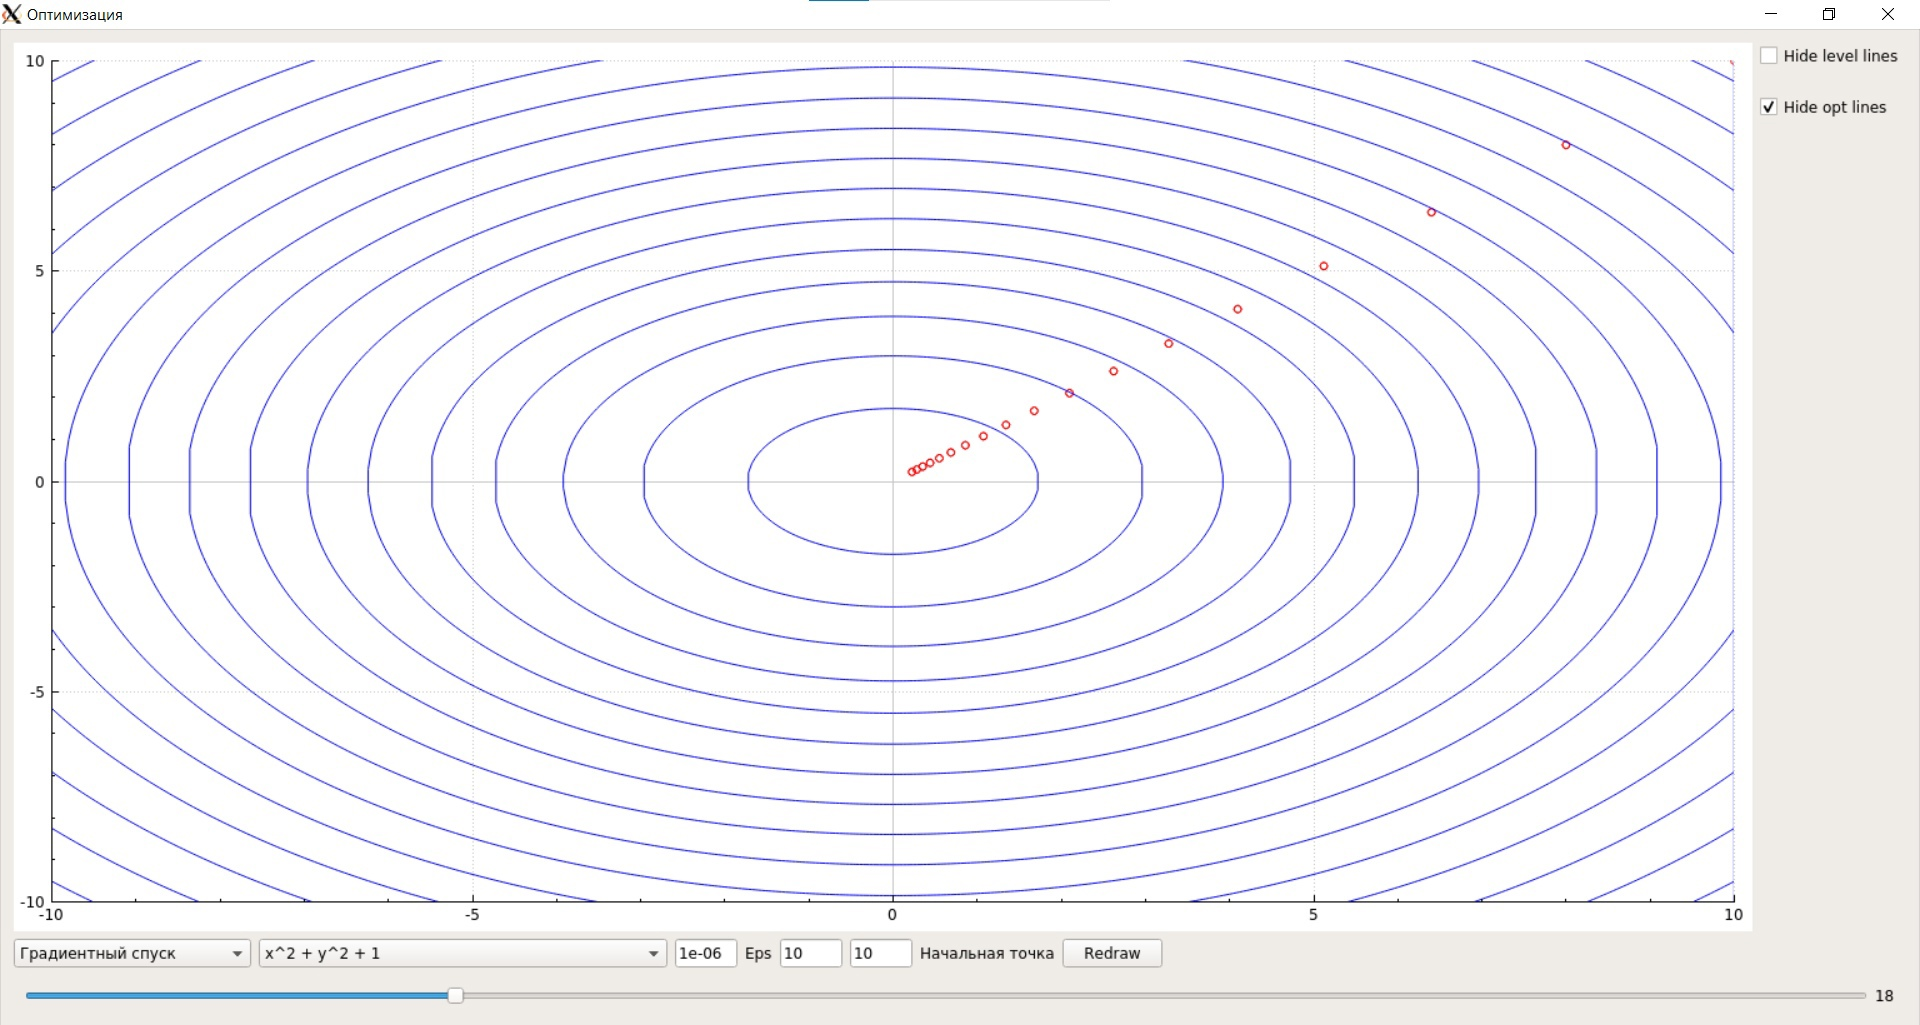
\includegraphics[scale=0.2]{img/gui.jpg}\\
	Графический интерфейс позволяет выбрать метод оптимизации функций, способ одномерного поиска для наискорейшего спуска, одну из четырех предложенных квадратичных функций, а также указать начальное приближение и стартовую точку.\\
	При передвижении ползунка внизу последовательно отображаются точки, вычисленные на каждой итерации.\\
	Изображение можно масштабировать и передвигать, справа есть вариант скрыть линии уровня и прямые, соединяющие точки.
	\newpage

	\section{Исходный код}
	
	\subsection{Диаграмма классов}
	\begin{figure}[h]
		\centering
		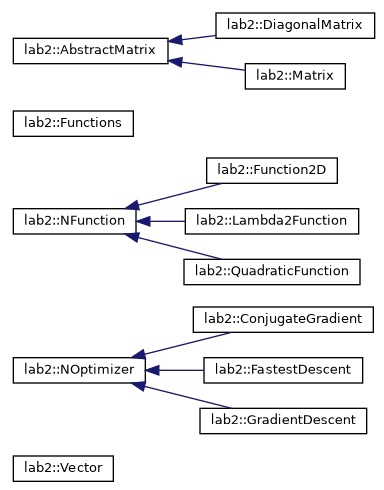
\includegraphics[scale=0.7]{img/diagram.jpg}
	\end{figure}
	\newpage
	
	\subsection{Вектор}
	\mcode{../../include/lab2/vector.h}
	\mcode{../../source/lab2/vector.cpp}
	\newpage
	
	\subsection{Общий класс матриц}
	\mcode{../../include/lab2/abstract_matrix.h}
	\mcode{../../source/lab2/abstract_matrix.cpp}
	\newpage
	
	\subsection{Матрица}
	\mcode{../../include/lab2/matrix.h}
	\mcode{../../source/lab2/matrix.cpp}
	\newpage
	
	\subsection{Диагональная матрица}
	\mcode{../../include/lab2/diagonal_matrix.h}
	\mcode{../../source/lab2/diagonal_matrix.cpp}
	\newpage
	
	\subsection{Функция}
	\mcode{../../include/lab2/n_function.h}
	\mcode{../../source/lab2/n_function.cpp}
	\newpage
	
	\subsection{Квадратичная функция}
	\mcode{../../include/lab2/quadratic_function.h}
	\mcode{../../source/lab2/quadratic_function.cpp}
	\newpage
	
	\subsection{Абстрактный класс оптимизатора}
	\mcode{../../include/lab2/n_optimizer.h}
	\mcode{../../source/lab2/n_optimizer.cpp}
	\newpage
	
	\subsection{Метод градиентного спуска}
	\mcode{../../include/lab2/gradient_descent.h}
	\mcode{../../source/lab2/gradient_descent.cpp}
	\newpage
	
	\subsection{Метод наискорейшего спуска}
	\mcode{../../include/lab2/fastest_descent.h}
	\mcode{../../source/lab2/fastest_descent.cpp}
	\newpage
	
	\subsection{Метод сопряженных градиентов}
	\mcode{../../include/lab2/conjugate_gradient.h}
	\mcode{../../source/lab2/conjugate_gradient.cpp}
	\newpage
	
	\subsection{Используемые функции}
	\mcode{../../include/lab2/functions.h}
	\mcode{../../source/lab2/functions.cpp}
	\newpage
	
\end{document}